\chapter{INTRODUÇÃO}\label{sec:introducao}

A estimação precisa das velocidades longitudinais e laterais desempenha papel importante em termos de segurança, estabilidade e eficiência operacional. Essas velocidades são fundamentais para o controle de veículos, especialmente em condições como curvas acentuadas, mudanças repentinas de direção e situações de emergência. Além disso, a determinação dessas velocidades permite calcular o ângulo de deriva, um parâmetro utilizado para avaliar a estabilidade direcional, prevenir acidentes e analisar o desempenho dinâmico \cite{wang2023}.

Métodos baseados em modelos físicos enfrentam obstáculos decorrentes da necessidade de uma modelagem detalhada do comportamento do veículo, levando em conta forças como o atrito dos pneus e os efeitos aerodinâmicos. Essa abordagem resulta em equações matemáticas complexas e não lineares, aplicadas em cenários dinâmicos \cite{singh2018}. A complexidade se eleva quando se considera condições como variações de terreno ou mudanças climáticas, situações em que os métodos tradicionais podem apresentar limitações para acompanhar a dinâmica do ambiente \cite{viehweger2020}.

Algoritmos de Inteligência Artificial (IA), como a Programação Genética Multigene (MGGP), destacam-se por evoluir múltiplos genes que se combinam para gerar expressões simbólicas capazes de modelar relações não lineares entre leituras de sensores e as velocidades longitudinal e lateral, sem exigir um modelo físico explícito \cite{mota2022}. Além disso, sensores virtuais baseados em dados podem utilizar sensores convencionais, como acelerômetros e giroscópios, reduzindo custos de implementação \cite{kong2022}. Estudos recentes indicam que ferramentas de IA podem atingir resultados comparáveis aos obtidos com sensores de custo elevado, posicionando-se como uma alternativa para veículos inteligentes e comerciais \cite{jin2021}.

Ao contrário de modelos baseados em estruturas de tipo caixa-preta, o MGGP utiliza a evolução simbólica para derivar expressões matemáticas que, além de capturarem relações não lineares entre os sinais de sensores --- como acelerômetros e giroscópios --- e as velocidades $v_x$ e $v_y$, mantêm um nível de interpretabilidade para a engenharia de controle \cite{olson2010, castro2023}.

Entre as grandezas que um sensor virtual pode fornecer, o ângulo de deriva ($\beta$) ocupa posição particular. Ele descreve a diferença entre a direção para a qual o veículo aponta e a direção em que de fato se desloca, e é uma das variáveis centrais dos sistemas de controle de estabilidade. Sua medição direta, contudo, exige sensores ópticos ou sistemas de posicionamento global e de navegação inercial (GPS/INS, do inglês \textit{Global Positioning System} e \textit{Inertial Navigation System}) de alto custo, o que motiva a sua estimação a partir de sensores embarcados convencionais \cite{chindamo2018, liu2018}.

Na Iniciação Científica (IC) que antecedeu este trabalho, foi desenvolvido um sensor virtual MGGP com cinco entradas e duas saídas, que estima simultaneamente $v_x$ e $v_y$. A partir dessas estimativas, o ângulo de deriva pode ser obtido diretamente por $\hat\beta = \operatorname{atan2}(\hat v_y, \hat v_x)$. Surge, então, a pergunta que motiva este Trabalho de Conclusão de Curso (TCC): estimar $\beta$ como uma terceira saída do próprio modelo de múltiplas entradas e múltiplas saídas (MIMO, do inglês \textit{Multiple-Input Multiple-Output}) --- de modo que o algoritmo evolutivo o considere durante o treinamento --- produz um ângulo de deriva mais preciso do que calculá-lo depois, a partir das velocidades estimadas? E essa terceira saída altera a qualidade das estimativas de $v_x$ e $v_y$? Como o MGGP ajusta todas as saídas com uma única função de aptidão e realimenta as estimativas de todas elas nas demais, a resposta não é evidente \emph{a priori}, e precisa ser medida.

\section{Objetivos}

O objetivo geral deste trabalho é estimar o ângulo de deriva de um veículo por meio de um sensor virtual simbólico baseado em Programação Genética Multigene, dando continuidade ao modelo desenvolvido na IC, e avaliar se a inclusão de $\beta$ como terceira saída do modelo MIMO melhora essa estimação em relação ao ângulo calculado a partir das velocidades estimadas.

Os objetivos específicos são:

\begin{alineas}
    \item comparar, em pistas não utilizadas no treinamento, o erro de $\beta$ obtido pela terceira saída evoluída de modelos com cinco entradas e três saídas (5×3) com o erro de $\beta$ pós-calculado a partir de modelos com cinco entradas e duas saídas (5×2);
    \item verificar se a terceira saída altera a qualidade das estimativas de $v_x$ e $v_y$ em relação aos modelos 5×2;
    \item comparar, dentro de um mesmo modelo 5×3, a saída evoluída de $\beta$ com o ângulo calculado a partir das velocidades que o próprio modelo estima;
    \item situar esses resultados em relação a um estimador cinemático de $\beta$ e aos modelos de referência da IC, e interpretar fisicamente as equações obtidas para $\beta$.
\end{alineas}

\section{Relação com a Iniciação Científica}

Este TCC reaproveita da IC a base de dados experimental, a biblioteca MGGP em Python, as entradas do sensor virtual e a configuração de hiperparâmetros que produziu o melhor modelo daquela pesquisa. Na IC, uma busca sistemática de 147 configurações estruturais --- sete valores de número de termos, sete de profundidade máxima das árvores e três janelas de atraso --- identificou como melhor configuração a de atrasos $[1, 2, 5, 10, 25, 50]$, sete termos por saída e profundidade máxima seis (denominada T48), com raiz do erro quadrático médio (RMSE, do inglês \textit{Root Mean Square Error}) média de 0,2121~m/s nas velocidades. A IC mostrou, ainda, que as equações obtidas recuperam a forma discreta das equações cinemáticas do modelo de bicicleta. A \autoref{fig:evolucao_ic} resume aquela busca: com um único atraso, muitas configurações divergiram em simulação livre, enquanto as janelas de atraso mais longas estabilizaram os modelos.

\begin{figure}[htbp]
    \centering
    \caption{RMSE médio dos modelos de cada treinamento da busca realizada na IC, por janela de atrasos.}
    \label{fig:evolucao_ic}
    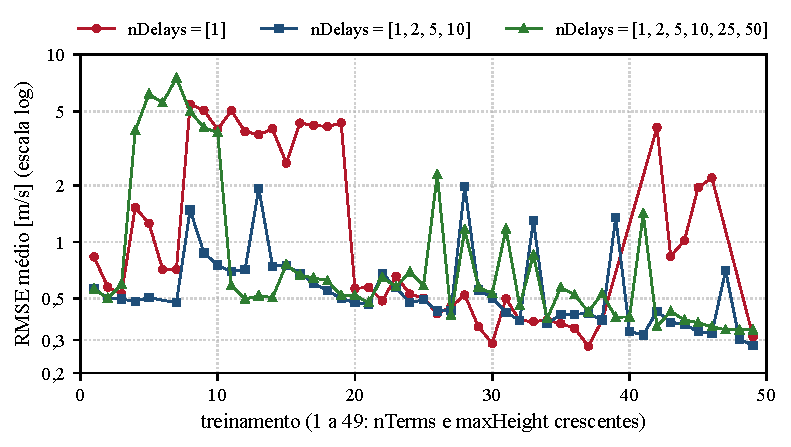
\includegraphics[width=\textwidth]{figuras/evolucao_ic.pdf}
    \fonte{Elaboração própria com dados da IC.}
\end{figure} Neste trabalho, essa configuração é mantida fixa, de modo que qualquer diferença observada entre os modelos 5×2 e 5×3 possa ser atribuída à terceira saída, e não a uma mudança de hiperparâmetros.